\section{Collaboration}

\begin{frame}
  \tableofcontents[currentsection]
\end{frame}

\begin{frame}{Collaboration}
  \begin{itemize}
    \item Jedes git Repository enthält die vollständige Versionshistorie
    \item Jeder Benutzer kann Repositories veröffentlichen (push)
    \item Unterstützte Protokolle:
    %http://progit.org/book/ch4-1.html
    \begin{itemize}
      \item file
      \item git
      \item http(s)
      \item ssh
    \end{itemize}
    \item Git unterstützt mehrere Entwicklungsmodelle (Distributed Workflows)
  \end{itemize}
\end{frame}

\begin{frame}[allowframebreaks]{Distributed Workflows}
  \framesubtitle{Centralized Workflow}
  \begin{figure}
    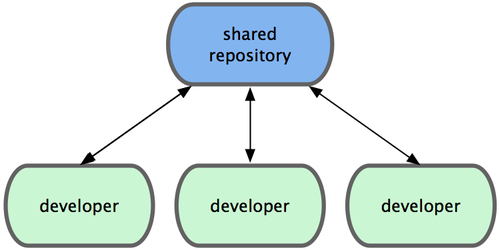
\includegraphics[width=0.5\textwidth]{img/wf-centralized}
    \caption[format=empty]{Quelle: \url{http://progit.org}}
  \end{figure}
  \framebreak
    
  \framesubtitle{Integration-Manager Workflow}
  \begin{figure}
    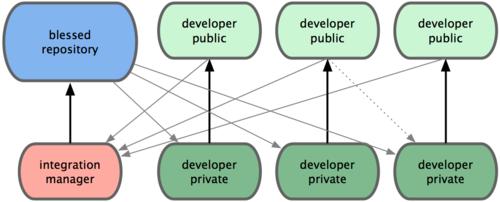
\includegraphics[width=0.6\textwidth]{img/wf-integration-manager}
    \caption[format=empty]{Quelle: \url{http://progit.org}}
  \end{figure}
  \framebreak

  \framesubtitle{Dictator and Lieutenants Workflow}
  \begin{figure}
   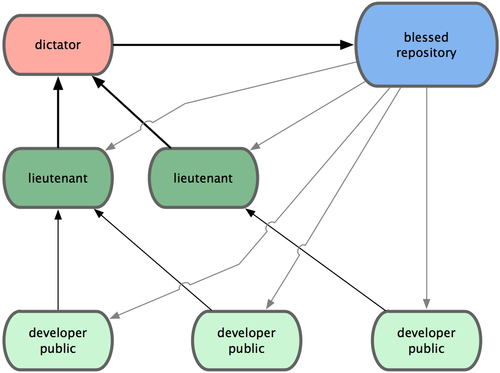
\includegraphics[width=0.5\textwidth]{img/wf-dictator}
    \caption[format=empty]{Quelle: \url{http://progit.org}}
  \end{figure}
\end{frame}

\begin{frame}[allowframebreaks]{Git Hosting}
  \begin{itemize}
    \item Github:
    \begin{itemize}
      \item Hosting unter: \url{http://github.com}
      \item Hohe Popularität
      \item Viele Features
      \item Quellcode nicht verfügbar
    \end{itemize}
    \item Gitorious:
    \begin{itemize}
      \item Hosting unter: \url{http://gitorious.org}
      \item Integrierte Benutzerverwaltung
      \item Freie Software (AGPL, \url{http://gitorious.org/gitorious})
    \end{itemize}
  \framebreak
    \item Gitosis:
    \begin{itemize}
      \item einfach, gut geeignet für kleineres Setup
      \item Freie Software (GPLv2, \url{http://eagain.net/gitweb/?p=gitosis.git})
    \end{itemize}
    \item Gitolite:
    \begin{itemize}
      \item komplex, aber sehr flexibel 
      \item Freie Software (GPLv2, \url{https://github.com/sitaramc/gitolite})
    \end{itemize}
  \end{itemize}
\end{frame}

% vim: tabstop=2 expandtab shiftwidth=2 softtabstop=2 autoindent
